\documentclass[10pt,slides,xcolor=pdftex,dvipsnames,table]{beamer}

%_ PACKAGES __________________________________________________________________________ %

    %__ INPUT/OUTPUT LANGUAGE _________________________________ %
    \usepackage[brazilian]{babel}
	\usepackage[utf8]{inputenc}
	\usepackage{lmodern}
	\usefonttheme{serif}

    %__ MATH __________________________________________________ %
    \usepackage{amssymb}
    \usepackage{amsmath}
    \usepackage{amsthm}
    \usepackage{bbm}
    \usepackage{amsfonts}
    \DeclareMathOperator*{\argmax}{argmax}
    
    \usepackage{cancel}

    %__ GRAPHS & TABLES________________________________________ %
    \usepackage{graphicx}
    \usepackage{booktabs}
    \usepackage{multirow}
    \usepackage{array}
    \usepackage{lscape}
    \usepackage{caption}
    \usepackage{tabularx}
    \usepackage{tabularx}
        \newcolumntype{Z}{>{\centering\arraybackslash}X}
        \newcolumntype{L}{>{\raggedright\arraybackslash}X}	
    
        \renewcommand{\arraystretch}{1.2}
%        \usepackage{subcaption}			% SUBFIGURE IS DEPRECATED; SHOULD USE SUBCAPTION INSTEAD OF .
    \usepackage[flushleft,online,para]{threeparttable}
    \usepackage{multirow}
    \usepackage{dcolumn}
        \newcolumntype{d}[1]{D{.}{\cdot}{#1}}
    \usepackage{rotating}                                      % for **sideways**tables

    %\usepackage[nolists]{endfloat}     %   PUTS FIGURES AT THE END OF DOCUMENT.
                                        %   DOESN'T WORK WITH \usepackage{float}


%	\usepackage{ulem}

  \usepackage{listings}
  \usepackage{xcolor}
      \definecolor{BackgroundGray}{cmyk}{0,0,0,.1}
      \definecolor{CommentGreen}{cmyk}{.26,0,.50,.68}
      \definecolor{CPIgraydark}{RGB}{104,102,100}
      \definecolor{black}{rgb}{0.1,0.1,0.1}
      \definecolor{pcolor}{rgb}{0.25,0.29,0.3}
        
\setbeamercolor{frametitle}{fg=black,bg=white}
\setbeamercolor{title}{fg=black,bg=white}

  \lstset{ %
    backgroundcolor=\color{BackgroundGray}, % choose the background color; you must add \usepackage{color} or \usepackage{xcolor}
    basicstyle=\ttfamily\tiny,                 % the size of the fonts that are used for the code
    breakatwhitespace=false,              % sets if automatic breaks should only happen at whitespace
    breaklines=true,                      % sets automatic line breaking
    captionpos=b,                         % sets the caption-position to bottom
    commentstyle=\color{CommentGreen},    % comment style
    deletekeywords={...},                 % if you want to delete keywords from the given language
    escapechar={\@},                      % if you want to add LaTeX within your code
    extendedchars=true,                   % lets you use non-ASCII characters; for 8-bits encodings only, does not work with UTF-8
    frame=none,                           % adds a frame around the code
    keepspaces=true,                      % keeps spaces in text, useful for keeping indentation of code (possibly needs columns=flexible)
    keywordstyle=\color{blue},           % keyword style
    language=R,                           % the language of the code
    morekeywords={*,...},                 % if you want to add more keywords to the set
    morestring=[b]",
    morestring=[d]',
    numbers=none,                         % where to put the line-numbers; possible values are (none, left, right)
    numbersep=5pt,                        % how far the line-numbers are from the code
    numberstyle=\tiny\color{gray},        % the style that is used for the line-numbers
    rulecolor=\color{black},              % if not set, the frame-color may be changed on line-breaks within not-black text (e.g. comments (green here))
    showspaces=false,                     % show spaces everywhere adding particular underscores; it overrides 'showstringspaces'
    showstringspaces=false,               % underline spaces within strings only
    showtabs=false,                       % show tabs within strings adding particular underscores
    stepnumber=2,                         % the step between two line-numbers. If it's 1, each line will be numbered
    stringstyle=\color{red},              % string literal style
    tabsize=2,                            % sets default tabsize to 2 spaces
    title=\lstname,                       % show the filename of files included with \lstinputlisting; also try caption instead of title
    columns=flexible
  }
\lstset{literate=
  {á}{{\'a}}1 {é}{{\'e}}1 {í}{{\'i}}1 {ó}{{\'o}}1 {ú}{{\'u}}1
  {Á}{{\'A}}1 {É}{{\'E}}1 {Í}{{\'I}}1 {Ó}{{\'O}}1 {Ú}{{\'U}}1
  {à}{{\`a}}1 {è}{{\`e}}1 {ì}{{\`i}}1 {ò}{{\`o}}1 {ù}{{\`u}}1
  {À}{{\`A}}1 {È}{{\'E}}1 {Ì}{{\`I}}1 {Ò}{{\`O}}1 {Ù}{{\`U}}1
  {ä}{{\"a}}1 {ë}{{\"e}}1 {ï}{{\"i}}1 {ö}{{\"o}}1 {ü}{{\"u}}1
  {Ä}{{\"A}}1 {Ë}{{\"E}}1 {Ï}{{\"I}}1 {Ö}{{\"O}}1 {Ü}{{\"U}}1
  {â}{{\^a}}1 {ê}{{\^e}}1 {î}{{\^i}}1 {ô}{{\^o}}1 {û}{{\^u}}1
  {Â}{{\^A}}1 {Ê}{{\^E}}1 {Î}{{\^I}}1 {Ô}{{\^O}}1 {Û}{{\^U}}1
  {Ã}{{\~A}}1 {ã}{{\~a}}1
  {œ}{{\oe}}1 {Œ}{{\OE}}1 {æ}{{\ae}}1 {Æ}{{\AE}}1 {ß}{{\ss}}1
  {ç}{{\c c}}1 {Ç}{{\c C}}1 {ø}{{\o}}1 {å}{{\r a}}1 {Å}{{\r A}}1
  {€}{{\EUR}}1 {£}{{\pounds}}1
}  
  %\DefineShortVerb{\|}

\setbeamertemplate{itemize item}{\color{black}$\blacktriangleright$}
\setbeamertemplate{itemize subitem}{\color{black}$\blacksquare$}

\setbeamercolor{enumerate item}{fg=black,bg=white}
\setbeamercolor{enumerate subitem}{fg=black,bg=white}

    %__ BIBLIOGRAPHY __________________________________________ %
    \usepackage[round,longnamesfirst]{natbib}

    %__ APPENDIX _____________________________________________ %
%    \usepackage[titletoc,page]{appendix}

    %__ PDF, DISPLAY & PRODUCTIVITY ___________________________ %
    \usepackage{hyperref}
    %\usepackage[textsize=footnotesize,colorinlistoftodos,textwidth=4cm,obeyDraft]{todonotes}
    \usepackage{pgfpages}
    \usepackage{pdfpages}    
%    \usepackage{pdfsync}
    \usepackage{pifont} % wtf?
%    \usepackage{bbding} % wtf?
    \usepackage{verbatim}

    \usepackage{wasysym} % smiley/frownie


%%%%%%%%%%%%%%%%%%%%%%%%%%%%%%%%%%%%%%%%%%%%%%%%%%%%%%%%%%%%%%%%%%%%%%%%%%%%

\beamertemplatenavigationsymbolsempty

    \newcommand{\mc}{\multicolumn}
    \newcommand{\lbar}{\underline}
    \newcommand{\ubar}{\overline}

    \newtheorem{resposta}{Resposta}
    \newtheorem{pergunta}{Pergunta}    


%%%%%%%%%%%%%%%%%%%%%%%%%%%%%%%%%%%%%%%%%%%%%%%%%%%%%%%%%%%%%%%%%%%%%%%%%%%%

%\AtBeginSection[] {
%  \begin{frame}[plain]
%    \frametitle{Chapters}
%    \tableofcontents[currentsection]
%  \end{frame}
%  \addtocounter{totalframenumber}{-1}
%}

\addtocounter{framenumber}{-1}
% FOOTLINE - PAGE NUMBER RIGHT
\defbeamertemplate*{footline}{guildford foot theme}
{
  \leavevmode%
  \hbox{%
  \begin{beamercolorbox}[wd=.7\paperwidth,ht=1cm,dp=0ex,left]{}%
    {
    \insertsectionnavigationhorizontal{.5\paperwidth}{}{}
    }
 \end{beamercolorbox}
 \begin{beamercolorbox}[wd=0.31\paperwidth,ht=1cm,dp=0ex,right]{}%
	{\tiny
	\insertframenumber{} / \inserttotalframenumber\hspace*{5ex}
	}
 \end{beamercolorbox}}%
  \vskip5pt%
}

% Titles will appear in Small Cap Serif

\usefonttheme{structuresmallcapsserif}

% -----------------------------------------
% Center the Frame Title
% -----------------------------------------

\setbeamertemplate{frametitle} {
\begin{centering}
\vspace{0.1in} \insertframetitle
\par
\end{centering}}

% -----------------------------------------
% Number the slides
% -----------------------------------------

\setbeamertemplate{footline}[frame number]

% -----------------------------------------
% Get rid of the irritating navigation bar
% -----------------------------------------

\setbeamertemplate{navigation symbols}{}

%------------------------------------------

\newenvironment{wideitemize}{\itemize\addtolength{\itemsep}{8pt}}{\enditemize}

\newcommand{\ind}{\perp\!\!\!\!\perp}

%%%%%%%%%%%%%%%%%%%%%%%%%%%%%%%%%%%%%%%%%%%%%%%%%%%%%%%%%%%%%%%%%%%%%%%%%%%%


%%%%%%%%%%%%%%%%%%%%%%%%%%%%%%%%%%%%%%%%%%%%%%%%%%%%%%%%%%%%%%%%%%%%%%%%%%%%
\title{
     Métodos Quantitativos I \\\vspace{6pt}
     Aula 6: Mínimos Quadrados Ordinários \\
    }
\author{Profs. Arthur Bragança e Daniel Grimaldi}
\institute{MPAM-ENAP}
\date{6 de agosto de 2025}


%%%%%%%%%%%%%%%%%%%%%%%%%%%%%%%%%%%%%%%%%%%%%%%%%%%%%%%%%%%%%%%%%%%%%%%%%%%%

\begin{document}

% - TITLE PAGE ---------------------------------------------------- %
    \begin{frame}[plain]
        \titlepage
    \end{frame}

    \begin{frame}[plain]
        \tableofcontents
    \end{frame}
    
% --------------------------------------------- END SLIDE --------- %

\section{Introdução}

%------------------------------------------------------------------ %

\begin{frame}{Introdução}

\begin{itemize}\itemsep1.2em

    \item Na aula passada estudamos os modelo de regressão bivariado e multivariado.
	
	\item Nessa aula:
	
	\begin{itemize}
	\item Estudaremos as propriedades dos estimadores de MQO.
	\item Estudaremos como testar hipóteses sobre os parâmetros de MQO.
	\item Discutiremos o que ocorre quando variância do termo de erro não é constante.
	\item Estudaremos as propriedades dos estimadores de MQO em amostras grandes.
	\item Discutiremos o que ocorre quando há correlação entre regressores e termo de erro.
	\end{itemize}

\end{itemize}

\end{frame}

%------------------------------------------------------------------ %

\section{Propriedades}

%------------------------------------------------------------------ %

\begin{frame}[fragile]
	\frametitle{Propriedades (1)}

\begin{itemize}\itemsep1.2em

\item \textbf{Mínimos Quadrados Ordinários (MQO)}: estimadores com propriedades desejáveis.

\item O que são propriedades desejáveis?
\begin{enumerate}
\item \textbf{Não viesado}: expectativa do estimador do parâmetro é igual ao parâmetro verdadeiro
\item \textbf{Eficiente}: variância do estimador é a menor possível     
\end{enumerate}        

\item Para ver essas propriedades iremos listar um conjunto de hipóteses.

\item Depois derivaremos a média e a variância do estimador. 

\end{itemize}

\end{frame}

%------------------------------------------------------------------ %

\begin{frame}[fragile]
	\frametitle{Propriedades}

\begin{itemize}\itemsep1.2em

\item \textbf{Hipóteses}:
\begin{enumerate}
\item \textbf{Modelo populacional:} o modelo populacional é
$$ y = X \beta;$$
\item \textbf{Amostragem aleatória:} $\left\{ (y_i, x_{i1},…, x_{ik}): i=1,...n \right\}$ é uma amostra independente e identicamente distribuída;
\item \textbf{Independência condicional}: $E[u | X ] = 0$;
\item \textbf{Variação em $X$:} $X = [X_1', \cdots X_n']'$ é matriz $n \times k$ com posto cheio;
\item \textbf{Homocedasticidade:} a variância o termo de erro é constante:
$$ V [u | X] = E [u u' | X] = \sigma^2 I $$ 
\end{enumerate}  

\item As hipóteses acima muitas vezes são chamadas de hipóteses de Gauss-Markov.
\begin{itemize}
\item Muitas vezes é adicionada a hipótese que $u | X \sim N(0, \sigma^2 I)$. 
\end{itemize}      

\end{itemize}

\end{frame}

%------------------------------------------------------------------ %

\begin{frame}[fragile]
	\frametitle{Média de $\widehat{\beta}$}

\begin{itemize}\itemsep1.2em

\item A média do estimador de MQO condicional a $X$ é

\begin{align*}
E [\widehat{\beta} | X] &= E \left[ (X'X)^{-1} X'y | X \right] \\
&= E \left[ (X'X)^{-1} X'(X \beta + u) | X \right] \\
&= \beta + (X'X)^{-1} X' E[u | X] \\ 
&= \beta 
\end{align*}

\item Lembre que $E[\widehat{\beta}] = E \left[E [\widehat{\beta} | X] \right]$.

\item Isso significa $E[\widehat{\beta}] = E \left[E [\widehat{\beta} | X] \right] = E[\beta]=\beta$.  

\item Logo, $\widehat{\beta}$ é um estimador não viesado de $\beta$.

\end{itemize}

\end{frame}

%------------------------------------------------------------------ %

\begin{frame}[fragile]
	\frametitle{Média de $\widehat{\beta}$ (bivariado)}

\begin{itemize}\itemsep1.2em

\item A média do estimador de MQO condicional a $x_i$ é

\begin{align*}
E [\widehat{\beta} | x_i] &= E \left[ \frac{\sum (x_i - \overline{x})(y_i - \overline{y})}{\sum (x_i - \overline{x})^2} | x_i \right] \\
&= E \left[ \frac{\sum (x_i - \overline{x})y_i}{\sum (x_i - \overline{x})^2} | x_i \right] - E \left[ \frac{\sum (x_i - \overline{x}) \overline{y}}{\sum (x_i - \overline{x})^2} | x_i \right] \\
&= E \left[ \frac{\sum (x_i - \overline{x}) (\alpha + \beta x_i + u_i) }{\sum (x_i - \overline{x})^2} | x_i \right] \\
&= \beta + E \left[ \frac{\sum (x_i - \overline{x}) u_i}{\sum (x_i - \overline{x})^2} | x_i \right] \\
&= \beta + \left[ \frac{\sum (x_i - \overline{x})}{\sum (x_i - \overline{x})^2} \right] E \left[ u_i | x_i \right] = \beta
\end{align*}

\item Isso significa $E[\widehat{\beta}] = E \left[E [\widehat{\beta} | x_i] \right] = E[\beta]=\beta$. 

\end{itemize}

\end{frame}

%------------------------------------------------------------------ %

\begin{frame}[fragile]
	\frametitle{Variância de $\widehat{\beta}$}

\begin{itemize}\itemsep1.2em

\item A variância de $\widehat{\beta}$ condicional a $X$ é:

\begin{align*}
V [\widehat{\beta} | X] &= E \left[ (\widehat{\beta} - \beta)(\widehat{\beta} - \beta)'| X \right] 
\end{align*}

\item Note que: 
\begin{align*}
& \widehat{\beta} = (X'X)^{-1} X'y = (X'X)^{-1} (X'X) \beta + (X'X)^{-1} X'u \\
& \Longrightarrow  \widehat{\beta} - \beta = (X'X)^{-1} X'u
\end{align*}

\item Portanto: 
\begin{align*}
V [\widehat{\beta} | X] &= E \left[ ((X'X)^{-1} X'u)((X'X)^{-1} X'u)'| X \right] \\
&= E \left[ (X'X)^{-1} X' uu' X (X'X)^{-1} | X \right] \\
&= (X'X)^{-1} X' E[u u'| X]  X (X'X)^{-1} \\
&= \sigma^2 (X'X)^{-1}
\end{align*}

\end{itemize}

\end{frame}

%------------------------------------------------------------------ %

\begin{frame}[fragile]
	\frametitle{Variância de $\widehat{\beta}$}

\begin{itemize}\itemsep1.2em

\item A lei da variância total diz: 

$$ V [\widehat{\beta} ] = E \left[ V[\widehat{\beta} | X ] \right] + V \left[ E[\widehat{\beta} | X] \right] $$

\item Temos: 

$$V \left[ E[\widehat{\beta} | X] \right] = V [ \beta] = 0$$

\item Logo, 

$$ V [\widehat{\beta} ] = E \left[ V[\widehat{\beta} | X ] \right] = \sigma^2 (X'X)^{-1}$$

\item Variância do estimador de MQO depende da variância do termo de erro (``variância residual de y'') e da variância dos regressores.

\end{itemize}

\end{frame}

%------------------------------------------------------------------ %

\begin{frame}[fragile]
	\frametitle{Variância de $\widehat{\beta}$ (bivariado)}

\begin{itemize}\itemsep1.2em

\item A variância de $\widehat{\beta}$ condicional a $x_i$ é:

\begin{align*}
V [\widehat{\beta} | x_i] = E \left[ (\widehat{\beta} - \beta)^2 | x_i \right] 
\end{align*}

\item Note que: 
\begin{align*}
& \widehat{\beta} = \frac{\sum_{i=1}^n (x_i - \overline{x}) (y_i - \overline{y})}{\sum_{i=1}^n (x_i- \overline{x})^2} = \beta + \frac{\sum_{i=1}^n (x_i- \overline{x}) u_i}{\sum_{i=1}^n (x_i- \overline{x})^2} \\
& \Longrightarrow  \widehat{\beta} - \beta = \frac{\sum_{i=1}^n (x_i - \overline{x}) u_i}{\sum_{i=1}^n (x_i- \overline{x})^2} = \sum_{i=1}^n w_i u_i
\end{align*}

\item Portanto: 
\begin{align*}
V [\widehat{\beta} | x_i] &= E \left[ \left( \sum_{i=1}^n w_i u_i \right)^2 | x_i \right] = E \left[ \left( \sum_{i=1}^n w_i^2 u_i^2 \right) | x_i \right] \\
&=  \sigma^2 \left(\sum_{i=1}^n w_i\right)^2 = \frac{\sigma^2}{\sum_{i=1}^n (x_i- \overline{x})^2} 
\end{align*}

\end{itemize}

\end{frame}

%------------------------------------------------------------------ %

\begin{frame}[fragile]
	\frametitle{Teorema de Gauss-Markov}

\begin{itemize}\itemsep1.2em

\item Se as hipóteses 1-5 são válidas, o estimador de MQO é o melhor estimador linear não viesado do vetor $\beta$.

\item O que isso significa? Considere a classe de estimadores lineares:

$$ \widetilde{\beta} = \sum_{i=1}^n W_i y_i, $$

em que $W_i$ é uma função da amostra.

\item Teorema de Gauss-Markov diz que $W_i = (X_i X_i')^-1 X_i$ é a função que:
\begin{enumerate}
\item ... faz com que $\widetilde{\beta}$ tenha a menor variância possível (``melhor'')
\item ... entre os estimadores  que $E[\widetilde{\beta}] = \beta$ (``não viesado'')   
\end{enumerate}      

\end{itemize}

\end{frame}

%------------------------------------------------------------------ %

\begin{frame}[fragile]
	\frametitle{Distribuição Normal}

\begin{itemize}\itemsep1.2em

\item \textbf{Hipótese adicional}:

$$u | X \sim N(0, \sigma^2 I)$$     

\item Essa hipótese adicional caracteriza o que chamamos de \textbf{modelo de regressão linear clássico}.

\item Ela implica que o estimador $\widehat{\beta}$ tem distribuição normal.

\item \textbf{Por quê?} 

\begin{align*}
& \widehat{\beta} = \beta + (X'X)^{-1} X'u \\
& u | X \sim N(0, \sigma^2 I) \Longrightarrow \widehat{\beta} \sim N(\beta, \sigma^2 (X'X)^{-1})
\end{align*}

\end{itemize}

\end{frame}

%------------------------------------------------------------------ %

\section{Inferência em MQO}

%------------------------------------------------------------------ %

\begin{frame}[fragile]
	\frametitle{Inferência Estatística (1)}

\begin{itemize}\itemsep1.2em

\item Considere o modelo populacional:

$$ y = X\beta + u$$ 

\item Como testar hipóteses sobre $\widehat{\beta}$?

\item Vimos que $(\widehat{\beta} - \beta) / \text{sd} (\widehat{\beta}) \sim N(0,1)$. 

\item Isso permite construir intervalos de confiança e testar hipóteses. 
\begin{itemize}
\item ... se conhecermos $\sigma^2$...
\item ... mas na prática precisamos estimar $\sigma^2$ 
\end{itemize}

\item O que fazer?

\end{itemize}

\end{frame}

%------------------------------------------------------------------ %

\begin{frame}[fragile]
	\frametitle{Inferência Estatística (2)}

\begin{itemize}\itemsep1.2em

\item Seja $\text{ep} (\widehat{\beta}) = \widehat{\sigma}^2 (X'X)^{-1}$ o erro-padrão dos estimadores de MQO.

\item Temos que

$$ (\widehat{\beta} - \beta) / \text{ep} (\widehat{\beta}) \sim t_{n-k-1} $$

em que $t_{n-k-1}$ é a distribuição t-Student com $n-k-1$ graus de liberdade.

\item Essa distribuição pode ser utilizada para testar hipóteses. 
\begin{itemize}
\item Essa distribuição converge para uma normal padronizada quando número de graus de liberdade tende a infinito (ex.: $> 120$). 
\end{itemize}

\end{itemize}

\end{frame}

%------------------------------------------------------------------ %

\begin{frame}[fragile]
	\frametitle{Inferência Estatística (3)}

\begin{itemize}\itemsep1.2em

\item Estimamos a variância dos erros com seguinte formula: 

\begin{align*}
 \widehat{\sigma^2} &= \frac{1}{n-k-1} \sum_{i=1}^n \widehat{u}_i^2 \\
&= \frac{1}{n-k-1} \sum_{i=1}^n \left( y_i - X_i' \widehat{\beta} \right)^2 \\
&= \frac{1}{n-k-1} (y-X\beta) (y-X\beta)' 
\end{align*}

\item Usar $n-k-1$, $n-k$ ou $n$ não faz diferença em grandes amostras. 
\begin{itemize}
\item Diferentes pacotes / opções no R utilizam diferentes denominadores.
\end{itemize}  

\end{itemize}

\end{frame}

%------------------------------------------------------------------ %

\begin{frame}[fragile]
	\frametitle{Teste de Hipóteses (1)}

\begin{itemize}\itemsep1.2em

\item Começamos considerando um teste cuja hipótese nula é 

$$H0: \beta_k = 0$$

\item Calculamos estatística $t_k = \beta_k/\text{ep} \left(\beta_k\right)$

\item Sob a hipótese nula, $t_k \sim N(0,1)$ (em amostras grandes)

\item \textbf{Regra de decisão:} rejeitamos H0 quando $t_k$ é tal que é improvável que hipótese nula seja verdadeira.
\begin{itemize}
\item $H1: \beta_k > 0$: H0 é rejeitada se $t_k$ é positivo e ``grande''
\item $H1: \beta_k < 0$: H0 é rejeitada se $t_k$ é negativo e ``grande''
\item $H1: \beta_k \neq 0$: H0 é rejeitada se $|t_k|$ é ``grande''
\end{itemize}     

\end{itemize}

\end{frame}

%------------------------------------------------------------------ %

\begin{frame}[fragile]
	\frametitle{Teste de Hipóteses (2)}

\begin{itemize}\itemsep1.2em

\item O que define ser ``grande'' é nível de significância adotado.

\item \textbf{Nível de significância:} probabilidade de rejeitar hipótese nula que é verdadeira

\item \textbf{Níveis típicos:} 10\%, 5\% e 1\% (5\% é o mais comum)

\item \textbf{p-valor}: qual o menor nível de significância para o qual eu não rejeitaria a hipótese nula?
\begin{itemize}
\item Inverte o cálculo.
\end{itemize}      

\end{itemize}

\end{frame}

%------------------------------------------------------------------ %

\begin{frame}[fragile]
	\frametitle{Teste de Hipóteses (3)}

\begin{center}
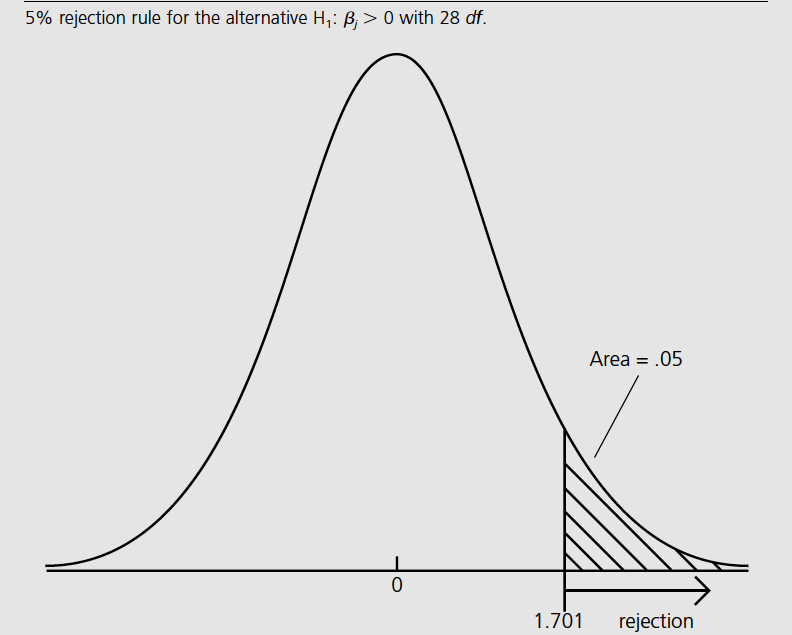
\includegraphics[height=0.8\textheight]{great0}
\end{center}

\end{frame}

%------------------------------------------------------------------ %

\begin{frame}[fragile]
	\frametitle{Teste de Hipóteses (4)}

\begin{center}
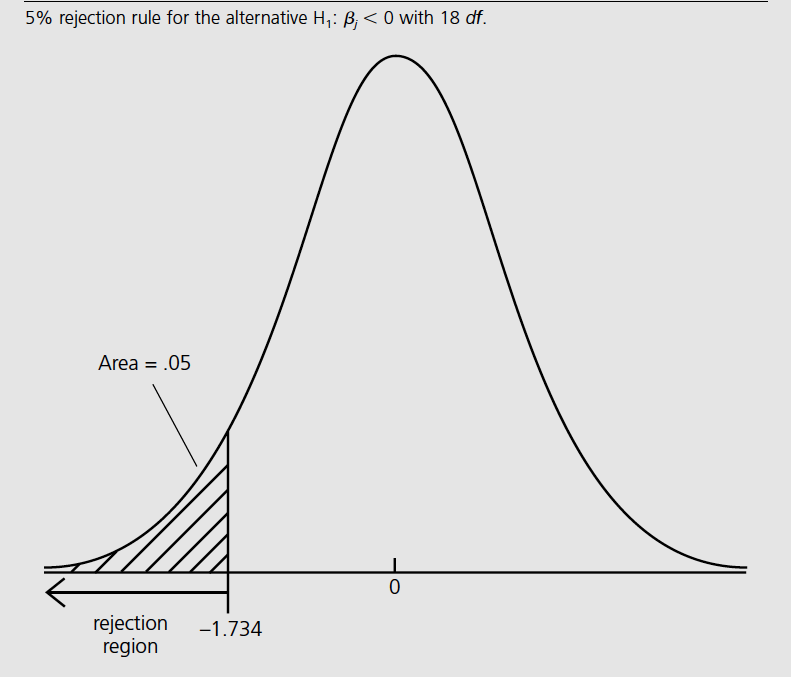
\includegraphics[height=0.8\textheight]{small0}
\end{center}

\end{frame}

%------------------------------------------------------------------ %

\begin{frame}[fragile]
	\frametitle{Teste de Hipóteses (5)}

\begin{center}
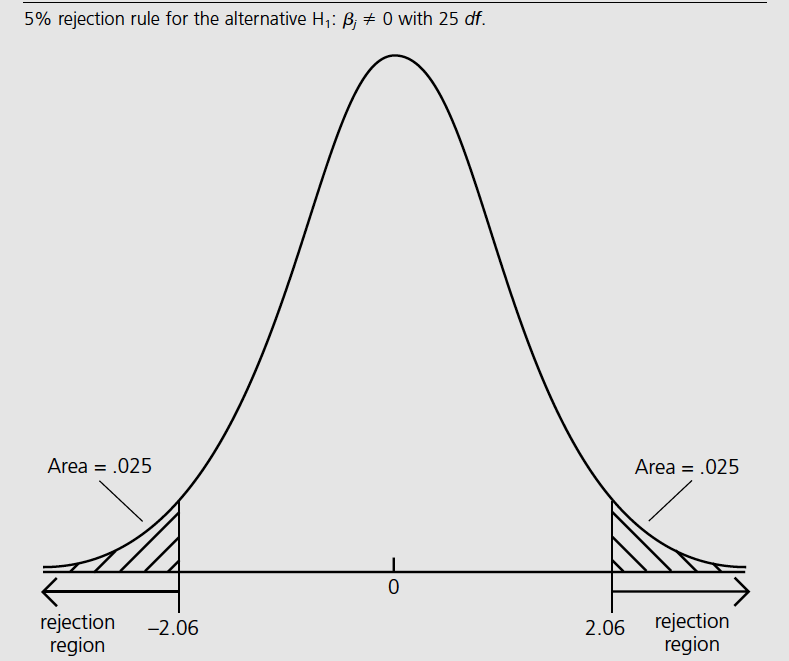
\includegraphics[height=0.8\textheight]{twosided}
\end{center}

\end{frame}

%------------------------------------------------------------------ %

\begin{frame}[fragile]
	\frametitle{Hipóteses Múltiplas (1)}

\begin{itemize}\itemsep1.2em

\item Muitas vezes estamos interessados em fazer testes sobre mais de um coeficiente.
\begin{itemize}
\item Coeficientes conjuntamente iguais a zero?
\item Soma de coeficientes é igual a um determinado valor?
\item Etc.
\end{itemize} 

\item \textbf{Ideia:}
\begin{itemize}
\item Constrói hipótese nula.
\item Roda modelo impondo que hipótese nula é verdadeira (modelo restrito)
\item Roda modelo sem impor que hipótese nula é verdadeira (modelo irrestrito)
\item Compara os modelos (como?). 
\end{itemize}

\end{itemize}

\end{frame}

%------------------------------------------------------------------ %

\begin{frame}[fragile]
	\frametitle{Hipóteses Múltiplas (2)}

\begin{itemize}\itemsep1.2em

\item Como comparar os modelos?

\item Podemos utilizar o $R2$ para construir estatística de teste.

$$ F = \frac{(R2_{ur} - R2_{r})/q}{(1- R2_{ur})/(n-k-1)} $$

em que $ur$ denota o modelo irrestrito, $r$ o modelo restrito e $q$ é o número de restrições sendo testadas 

\item A estatística F tem distribuição F-Snedecor com $q$ graus de liberdade no numerador e $n-k-1$ no denominador.

\item Logo, podemos utilizar essa distribuição para testar hipóteses múltiplas.

\end{itemize}

\end{frame}

%------------------------------------------------------------------ %

\begin{frame}[fragile]
	\frametitle{Hipóteses Múltiplas (3)}

\begin{itemize}\itemsep1.2em

\item Considere o modelo: 

$$ \log w_i = \beta_0 + \beta_1 \text{educ}_i + \beta_2 \text{age}_i + \beta_3 \text{age}_i^2 + u_i $$

\item Suponha que queremos testar $H0: \beta_2 = \beta_3 = 0$. 

\item Rodamos modelo restrito: 

$$ \log w_i = \beta_0 + \beta_1 \text{educ}_i + u_i $$ 

e computamos $R2_r$.

\item Depois rodamos modelo completo e computamos $R2_{ur}$.

\item Usamos os coeficientes de ajustes para construir estatística $F$ (note que $k=4$ e $q = 2$).  

\end{itemize}

\end{frame}

%------------------------------------------------------------------ %

\begin{frame}[fragile]
	\frametitle{Hipóteses Múltiplas (4)}

\begin{itemize}\itemsep1.2em

\item Comando \textbf{linearHypothesis()} permite testar hipóteses múltiplas.

\end{itemize}

\begin{lstlisting}

  #	Instala e carrega pacote #
  
  	install.packages("car")
  	
  	library(car)

  # Testando significancia conjunta # 
    
    modelo = lm_robust(lwage ~ educ + age + age2 + female + white, data = twins, se_type = "classical") # modelo que queremos analisar #
    
    hipotese.nula <- c("age=0", "age2=0") # hipotese conjunta a ser testada #
    
    linearHypothesis(modelo, hipotese.nula, test = "F") # teste F #

\end{lstlisting}

\end{frame}

%------------------------------------------------------------------ %

\section{Heterocedasticidade}

%------------------------------------------------------------------ %

\begin{frame}[fragile]
	\frametitle{Heterocedasticidade (1)}

\vspace{0.3cm}
Problema! Variância do erro não é constante.

\begin{lstlisting}

  # Estimo modelo lm_robust() # 
    
   modelo = lm_robust(lwage ~ educ + age + age2 + female + white, data = twins, se_type = "classical")    
   
  # Computo erros # 
   
  twins$erro = modelo$residuals 
  
  # regressor x erros (ou var. dep.) 
  
  plot(twins$educ,twins$erro)  
  
  plot(twins$educ,twins$lwage)
	
  plot(twins$age,twins$erro)  
  
  plot(twins$age,twins$lwage)	

\end{lstlisting}

Erros padrão robustos a heterocedasticidade dados por:

$$ V \left( \widehat{\beta} \right) = (X'X)^{-1} X' E[\hat{u} \hat{u}' | X] X (X'X)^{-1} $$ 

\end{frame}

%------------------------------------------------------------------ %

\begin{frame}[fragile]
	\frametitle{Heterocedasticidade (2)}

\vspace{0.3cm}
Pacote \textbf{lm\_robust} estima automaticamente erros-padrão robustos a heterocedasticidade.

\begin{lstlisting}

  # Estimo modelo com erro-padrão robusto # 
    
   modelo = lm_robust(lwage ~ educ + age + age2 + female + white, data = twins, se_type = "HC1")    
  
  
  # Opção type = "" do comando controla formula utilizada "

\end{lstlisting}

Diferentes opções do comando denotam diferentes ajustes de graus de liberdade na estimação da matriz de variância $E[\hat{u} \hat{u}' | X]$.

\vspace*{0.2cm}

\textbf{Problema!} Mínimos quadrados ordinários deixa de ser eficiente.

\end{frame}

%------------------------------------------------------------------ %

\begin{frame}[fragile]
	\frametitle{Heterocedasticidade (3)}

\begin{itemize}\itemsep1.2em

\item Mínimos Quadrados Generalizados: opção eficiente. 

\item Considere que 

$$ V [u | X] = \sigma^2 h(X) $$

\item Note que 

$$ V \left[ u / \sqrt{h(X)} | X \right] = \sigma^2$$

\item Estimador eficiente obtido regredindo $y/h(X)$ em $x/h(X)$.

\item \textbf{Dois casos:}
\begin{itemize}
\item $h(X)$ é conhecido: estimação direta
\item $h(X)$ não é conhecido: roda MQO, computa $\hat{h}(X)$ e estima novamente.
\end{itemize}

\end{itemize}

\end{frame}

%------------------------------------------------------------------ %

\section{MQO em grandes amostras}

%------------------------------------------------------------------ %

\begin{frame}[fragile]
	\frametitle{MQO em grandes amostras}

\begin{itemize}\itemsep1.2em 

\item Considere o modelo:

$$ y = X \beta + u $$

\item Derivamos as propriedades de $\widehat{\beta}$ em amostras finitas.       

\item Mas, mais e mais, obtemos $\widehat{\beta}$ em amostras cada vez maiores.

\item Quais as propriedades dos estimadores de MQO quando o número de observações cresce arbitrariamente ($n \rightarrow \infty$)?  

\end{itemize}

\end{frame}

%------------------------------------------------------------------ %

\begin{frame}[fragile]
	\frametitle{Consistência (1)}

\begin{itemize}\itemsep1.2em 

\item $\widehat{\beta}$ é um estimador consistente de $\beta$.

$$ \text{plim} (\widehat{\beta}) = \beta $$  
 
\item \textbf{Intuição:} à medida que amostra cresce o vetor de parâmetros estimados fica cada vez mais próximo que o vetor de parâmetros verdadeiro.

\item \textbf{Prova:}
\begin{align*}
& \widehat{\beta} = \beta + (X'X)^{-1} X'u = \beta + \left( \frac{1}{n} \sum_{i=1}^n (X_i X_i')^{-1} \right) \left( \frac{1}{n} \sum_{i=1}^n (X_i u_i) \right) \\
\\
& \Longrightarrow \text{plim} (\widehat{\beta}) = \beta + E[X_i X_i']^{-1} E [X_i u_i] = \beta, \, \text{pois} \, E [X_i u_i] = 0
\end{align*}


\end{itemize}

\end{frame}

%------------------------------------------------------------------ %

\begin{frame}[fragile]
	\frametitle{Consistência (2)}

\begin{itemize}\itemsep1.2em 

\item Note que consistência depende da covariância entre regressores e termo de erro ser zero ($E [X_i u_i] = 0$). 

\item Essa hipótese é implicada pela hipótese de média do termo de erro ser independente dos regressores ($E [u_i | X_i] = 0$).

\item Mas a recíproca não é verdadeira! (hipótese mais fraca)

\item Consistência ($\sim$ ausência de viés assintótico) depende de hipóteses mais fracas que ausência de viés.    

\end{itemize}

\end{frame}

%------------------------------------------------------------------ %

\begin{frame}[fragile]
	\frametitle{Normalidade Assintótica}

\begin{itemize}\itemsep1.2em 

\item A distribuição de $(\widehat{\beta} - \beta)/ \text{ep} (\widehat{\beta})$ converge para uma distribuição $N(0,1)$.  

\item Isso é uma aplicação do teorema central do limite. 
\begin{itemize}
\item Não depende de normalidade do termo de erro ($u_i$).
\item Só precisamos de que média do erro seja zero e sua variância finita. 
\end{itemize} 

\item \textbf{Implicação:} não precisamos impor normalidade para testar hipóteses em grandes amostras. 

\end{itemize}

\end{frame}

%------------------------------------------------------------------ %

\section{Problemas com MQO}

%------------------------------------------------------------------ %

\begin{frame}{O que ocorre quando $E[X_i u_i] \neq 0$?}

\begin{itemize}\itemsep1.2em

    \item Hipótese $E [X_i u_i] = 0$ é a principal hipótese de identificação do modelo de MQO.  
    
    \item O que ocorre se ela falha? 
    
    $$ \text{plim} (\widehat{\beta}) = \beta + E [ X_i X_i']^{-1} E[X_i u_i] $$
    
    \item $E[X_i u_i] \neq 0$ implica que $\text{plim} (\widehat{\beta}) \neq \beta$
    \begin{itemize}
    \item $E[X_i u_i] > 0$: MQO sobrestima parâmetro real
    \item $E[X_i u_i] < 0$: MQO subestima parâmetro real
    \end{itemize}
    
	\item Três casos em que $E[X_i u_i] \neq 0$: viés de variável omitida, viés de simultaneidade e viés de atenuação.       
        
\end{itemize}

\end{frame}

%------------------------------------------------------------------ %

\begin{frame}{Viés de Variável Omitida (1)}

\begin{itemize}\itemsep1.2em

    \item Hipótese $E [X_i u_i] = 0$ é a hipótese de identificação do modelo de MQO.  
    
    \item O que ocorre se ela falha? Considere o modelo:
    
    $$ y_i = \beta_0 + \beta_1 x_{1i} + \beta_2 x_{2i} + u_i, E[x_{1i} u_i]= E [x_{2i} u_i ] =0 $$

	\item Suponha que observamos $x_1$, mas não $x_2$ e considere a regressão de $y_i$ em $x_{1i}$. 
	
	\item Defina $\nu_i = \beta_2 x_{2i} + u_i$ e note que:
	
	$$ E [ x_{1i} \nu_i ] \neq 0 $$
        
\end{itemize}

\end{frame}

%------------------------------------------------------------------ %

\begin{frame}{Viés de Variável Omitida (2)}

\begin{itemize}\itemsep1.2em 
	
	\item Coeficiente da regressão de $y_i$ em $x_{1i}$ é: 
	
	$$ \hat{\beta_1} = \frac{cov (x_{1i},y_i)}{var(x_{1i})} $$
	
	\item Temos: 
	
	$$ \hat{\beta_1} = \frac{cov (x_{1i},\beta_1 x_{1i} + \beta_2 x_{2i} + u_i )}{var(x_{1i})} = \beta_1 + \beta_2 \frac{cov (x_{1i},x_{2i})}{var(x_{1i})} $$
	
	\item Efeito de MQO é efeito real mais produto entre efeito da variável omitida sobre $y$ e efeito de $x_1$ em $x_2$. 
	
	\item O viés que surge quando omitimos regressores relevantes é denominado viés de variável omitida.
	
	\item \textbf{Desafio}: garantir que não existem regressores relevantes não omitidos.
        
\end{itemize}

\end{frame}

%------------------------------------------------------------------ %

\begin{frame}{Exemplo}

\begin{itemize}\itemsep1.2em

\item Relação entre $y$ e os regressores $x_1$ e $x_2$ seja descrita pelo modelo populacional:

$$ y = \beta_0 + \beta_1 x_1 + \beta_2 x_2 + u $$

\item Relação entre $x_1$ e $x_2$ é descrita por:

$$ x_2 = \alpha x_1 + \nu $$

\item Suponha que os parâmetros populacionais sejam $\beta_0 = 0.1$, $\beta_1 = 0.6$, $\beta_2 = 0.4$ e $\alpha = 0.5$ e as distribuições $u \sim N(0,4)$, $\nu \sim N(0,16)$ e $x_1 \sim N(0,1)$.

\end{itemize}

\end{frame}

%------------------------------------------------------------------ %

\begin{frame}[fragile]
	\frametitle{Regressão Longa}

\vspace{0.5cm}
Simulo 10.000 observações dos vetores $u$, $\nu$, $x_1$, $x_2$ e $y$.

\begin{lstlisting}

  # Vetores # 
    
	set.seed(1985)
   
	beta0 = 0.1

	beta1 = 0.6
   
	beta2 = 0.4
 
	alpha = 0.5
   
	u = rnorm(10000, mean = 0, sd = 2)
 
	v = rnorm(10000, mean = 0, sd = 4)

	x1 = rnorm(10000, mean = 0, sd = 1)
 
	x2 = alpha*x1+v
 
	y = beta0 + beta1*x1 + beta2*x2 + u
  
	dados = data.frame(cbind(y,x1,x2))

\end{lstlisting}

\end{frame}

%------------------------------------------------------------------ %

\begin{frame}[fragile]
	\frametitle{Regressão Longa}

\vspace{0.5cm}
Rodo regressão longa.

\begin{lstlisting}

  # Regressão # 
    
	full.model = lm_robust(y ~ x1 + x2, data = dados, se_type = "HC1")
	
	summary(full.model)

Standard error type:  HC1 

Coefficients:
            Estimate Std. Error t value   Pr(>|t|) CI Lower CI Upper   DF
(Intercept)  0.06576   0.019964   3.294  9.915e-04  0.02663   0.1049 9997
x1           0.61181   0.020065  30.491 2.504e-195  0.57248   0.6511 9997
x2           0.39489   0.005066  77.950  0.000e+00  0.38496   0.4048 9997

Multiple R-squared:  0.4366 ,	Adjusted R-squared:  0.4364 
F-statistic:  3858 on 2 and 9997 DF,  p-value: < 2.2e-16

\end{lstlisting}

\end{frame}

%------------------------------------------------------------------ %

\begin{frame}[fragile]
	\frametitle{Regressão Curta}

\vspace{0.5cm}
Rodo regressão curta.

\begin{lstlisting}

	short.model = lm_robust(y ~ x1, data = dados, se_type = "HC1")

	summary(short.model)

Standard error type:  HC1 

Coefficients:
            Estimate Std. Error t value   Pr(>|t|)  CI Lower CI Upper   DF
(Intercept)  0.04258    0.02536   1.679  9.323e-02 -0.007139   0.0923 9998
x1           0.80015    0.02548  31.405 1.475e-206  0.750209   0.8501 9998

Multiple R-squared:  0.08995 ,	Adjusted R-squared:  0.08986 
F-statistic: 986.3 on 1 and 9998 DF,  p-value: < 2.2e-16

\end{lstlisting}

\end{frame}

%------------------------------------------------------------------ %

\begin{frame}{Viés de Simultaneidade (1)}

\begin{itemize}\itemsep1.2em

\item Considere o modelo de oferta e demanda:
\vspace{0.3cm}

$ \log Q_D = c_D + \epsilon_D \log P +  X_D' \gamma_D + \varepsilon_D $

\vspace{0.2cm}

$ \log P = c_S + \epsilon_S \log Q_S +  X_S' \gamma_S + \varepsilon_S $

\vspace{0.2cm}

$ \log Q^* = \log Q_D = \log Q_S $

\item Queremos estimar $\epsilon_D$ (elasticidade-preço da demanda) e $\epsilon_S$ (elasticidade preço da oferta).

\item Note que:
\vspace{0.3cm}

$  \log Q = c_D + \epsilon_D (c_S + \epsilon_S \log Q +  X_S' \gamma_S + \varepsilon_S) +  X_D' \gamma_D + \varepsilon_D \Longrightarrow E[\log Q \times \varepsilon_S] \neq 0 $

\vspace{0.3cm}

$  \log P = c_S + \epsilon_S (c_D + \epsilon_D \log P +  X_D' \gamma_D + \varepsilon_D) +  X_S' \gamma_S + \varepsilon_S \Longrightarrow E[\log P \times \varepsilon_D] \neq 0 $
        
\end{itemize}

\end{frame}

%------------------------------------------------------------------ %

\begin{frame}{Viés de Simultaneidade (2)}

\begin{itemize}\itemsep1.2em

\item O modelo de oferta e demanda ilustra como a estimação de mínimos quadrados ordinários (MQO) falha quando existe simultaneidade ou causalidade reversa.

\item $E[\log P \times \varepsilon_D] > 0$: MQO viesa elasticidade-preço da demanda para cima (i.e., em direção a zero).

\item $E[\log Q \times \varepsilon_S] < 0$: MQO viesa elasticidade-preço da oferta para baixo (em direção a zero).

\item \textbf{Exercício}: prove os fatos acima.    
        
\end{itemize}

\end{frame}

%------------------------------------------------------------------ %

\begin{frame}{Viés de Atenuação (1)}

\begin{itemize}\itemsep1.2em

\item Considere o modelo de regressão linear:

$$ y_i = \alpha + \beta x_i + \varepsilon, E[ \varepsilon | x_i]=0 $$

\item Suponha que $x_i$ não é observado e sim $x_i^* = x_i + \nu_i$.  Modelo estimado é:  

$$ y_i = \alpha + \beta x_i^* + (-\beta \nu_i + \varepsilon) $$

\item Defina $\text{var} (x_i) = \sigma_x^2$, $\text{var} (\varepsilon) = \sigma_u^2$, $\text{var} (\nu_i) = \sigma_{\nu}^2$ . Temos: 

$$ \beta_{MQO} = \frac{\text{cov} (x_i^*, y_i)}{\text{var} (x_i^*)} = \frac{\text{cov} (x_i^*, \alpha + \beta x_i^* - \beta \nu_i + \varepsilon)}{\text{var} (x_i^*)} $$

$$ = \beta - \beta \frac{\text{cov} (x_i+\nu_i, \nu_i) }{\text{var} (x_i + \nu_i)} = \beta - \beta \frac{\sigma_{\nu}^2}{\sigma_x^2 + \sigma_{\nu}^2} = \beta \left( \frac{\sigma_x^2}{\sigma_x^2 + \sigma_{\nu}^2} \right) < \beta $$
        
\end{itemize}

\end{frame}

%------------------------------------------------------------------ %

\begin{frame}{Viés de Atenuação (2)}

\begin{itemize}\itemsep1.2em

\item Considere o seguinte modelo populacional:

$$ y = \beta_0 + \beta_1 x + \varepsilon $$

\item Suponha que não observamos $x$ e sim $x^* = x + \nu$.

\item Os parâmetros populacionais são $\beta_0 = 1$ e $\beta_1 = 0.6$ 

\item $x$ tem distribuição $N(0,4)$

\item Os termos de erro $\nu$ e $\varepsilon$ tem distribuições $N(0,1)$ e $N(0,16)$, respectivamente. 

\end{itemize}

\end{frame}

%------------------------------------------------------------------ %

\begin{frame}[fragile]
	\frametitle{Viés de Atenuação (3)}

\vspace{0.5cm}
Simulo 10.000 observações dos vetores $u$, $\nu$, $x$, $x^*$ e $y$.

\begin{lstlisting}

  # Vetores # 
    
	set.seed(1985)
   
	beta0 = 1

	beta1 = 0.6

	x = rnorm(10000, mean = 0, sd = 2)
 
	v = rnorm(10000, mean = 0, sd = 1)

	u = rnorm(10000, mean = 0, sd = 4)
 
	y = beta0 + beta1*x + u
	
	xs = x + v
  
	dados = data.frame(cbind(y,x,xs))

\end{lstlisting}

\end{frame}

%------------------------------------------------------------------ %

\begin{frame}[fragile]
	\frametitle{Viés de Atenuação (4)}

\vspace{0.5cm}
Viés de atenuação: $\sigma_x^2/(\sigma_x^2 + \sigma_{\nu}^2) \times \beta = 0.8 \times 0.6 = 0.48$ 

\begin{lstlisting}

  # Vetores # 
    
library(estimatr)
 
summary(lm_robust(y ~ x, data = dados))

Coefficients:
            Estimate Std. Error t value   Pr(>|t|) CI Lower CI Upper   DF
(Intercept)   1.0367    0.03987   26.01 2.520e-144   0.9586   1.1149 9998
x             0.6093    0.01986   30.68 1.129e-197   0.5704   0.6483 9998

Multiple R-squared:  0.08515 ,	Adjusted R-squared:  0.08506 
F-statistic: 941.5 on 1 and 9998 DF,  p-value: < 2.2e-16

summary(lm_robust(y ~ xs, data = dados))

Coefficients:
            Estimate Std. Error t value   Pr(>|t|) CI Lower CI Upper   DF
(Intercept)   1.0397    0.04027   25.82 2.231e-142   0.9608   1.1186 9998
xs            0.4857    0.01817   26.73 4.293e-152   0.4501   0.5213 9998

Multiple R-squared:  0.0669 ,	Adjusted R-squared:  0.06681 
F-statistic: 714.5 on 1 and 9998 DF,  p-value: < 2.2e-16

\end{lstlisting}

\end{frame}

%------------------------------------------------------------------ %

%%------------------------------------------------------------------ %
%
%\section{Variáveis Instrumentais}

%%------------------------------------------------------------------ %
%
%\begin{frame}{Variáveis Instrumentais}
%
%\begin{itemize}\itemsep1.2em
%
%    \item Vimos três casos em que $E[X_i u_i] \neq 0$. O que fazer nesses casos?     
%    
%    \item Solução! Instrumento $Z_i$ (dimensão $l \times 1$) que cumpre duas condições:
%    
%    \begin{enumerate}\itemsep1.2em
%    
%	\item \textbf{Relevância}: $\text{cov} ( X_i, Z_i) \neq 0$ ($Z_i$ afeta $X_i$)
%	
%	\item \textbf{Exclusão}: $E [Z_i u_i] = 0$ ($Z_i$ só afeta $Y_i$ via $X_i$)   
%    
%    \end{enumerate}
%    
%    \item Tipicamente estimado em dois estágios (mas há outras maneiras de estimar!)
%     
%\end{itemize}
%
%\end{frame}
%
%%------------------------------------------------------------------ %
%
%\begin{frame}{Oferta e Demanda (1)}
%
%Considere o modelo de oferta e demanda:
%
%$$ \log Q_D = c_D + \epsilon_D \log P + \varepsilon_D $$
%
%$$ \log P = c_S + \epsilon_S \log Q_S + \gamma Z + \varepsilon_S $$
%
%$$ \log Q^* = \log Q_D = \log Q_S $$
%
%Queremos estimar $\epsilon_D$ (elasticidade-preço da demanda). Entretanto, $ E [ \log P,  \varepsilon_D ] \neq 0 $.
%
%\vspace{0.3cm}
%
%\textbf{Ideia}: utilizar $Z$ como instrumento de $P$ -- afeta preço (relevância) e não afeta quantidade a não ser através do seu efeito via preços (exclusão). 
%
%\end{frame}
%
%%------------------------------------------------------------------ %
%
%\begin{frame}{Oferta e Demanda (2)}
%
%\textbf{Exemplo}: Mercado de Peixes de Fulton (NY) (ver Graddy, K. (2006). Markets: The Fulton Fish Market. \textit{Journal of Economic Perspectives}, 20(2), 207-220.)
%
%\vspace{0.3cm}
%
%Queremos estimar elasticidade-preço da demanda por peixes.  
%
%\vspace{0.3cm}
%
%Instrumento ($Z$) são condições climáticas (choque de custos -- relacionado com preços e não relacionado com a demanda). 
%
%\vspace{0.3cm}
%
%Controles de dia da semana e tendências de tempo. 
% 
%
%\end{frame}
%
%%------------------------------------------------------------------ %
%
%\begin{frame}[fragile]
%	\frametitle{Estimação}
%
%\begin{lstlisting}
%
%# abre dados #
%
%dados = read.dta13("fish.dta")
%
%# MQO $
%
%modeloMQO = lm_robust(log(quantity) ~ log(price) + mon + tues + wed + thurs + time, data = dados)
%
%summary(modeloMQO)
%
%Coefficients:
%             Estimate Std. Error t value Pr(>|t|)    
%(Intercept)  8.301071   0.202785  40.935  < 2e-16 ***
%log(price)  -0.548897   0.184138  -2.981  0.00370 ** 
%mon         -0.317546   0.227223  -1.398  0.16570    
%tues        -0.683626   0.223630  -3.057  0.00294 ** 
%wed         -0.535288   0.220901  -2.423  0.01739 *  
%thurs        0.068269   0.221377   0.308  0.75850    
%time        -0.001250   0.002641  -0.473  0.63723    
%---
%
%Multiple R-squared:  0.2188,	Adjusted R-squared:  0.1667 
%
%\end{lstlisting}
%
%\end{frame}
%
%%------------------------------------------------------------------ %
%
%\begin{frame}[fragile]
%	\frametitle{MQ2E (1)}
%	
%\vspace{0.5cm}
%No procedimento de MQ2E (minímos quadrados de dois estágios) o primeiro estágio é uma regressão da variável endógena no instrumento.	
%
%\begin{lstlisting}
%
%# primeiro estágio - instrumento é tamanho das ondas #
%
%modelo1 = lm_robust(log(price) ~ wave2 + mon + tues + wed + thurs + time, data = dados)
%
%summary(modelo1)
%
%Standard error type:  HC2 
%
%Coefficients:
%             Estimate Std. Error  t value  Pr(>|t|)  CI Lower   CI Upper DF
%(Intercept) -0.705637   0.159035 -4.43699 2.577e-05 -1.021587 -0.3896859 90
%wave2        0.102781   0.020739  4.95587 3.361e-06  0.061579  0.1439835 90
%mon         -0.036482   0.116962 -0.31191 7.558e-01 -0.268846  0.1958829 90
%tues         0.007216   0.125654  0.05743 9.543e-01 -0.242418  0.2568493 90
%wed          0.082508   0.115595  0.71377 4.772e-01 -0.147141  0.3121576 90
%thurs        0.136126   0.106593  1.27706 2.049e-01 -0.075640  0.3478917 90
%time        -0.002107   0.001309 -1.60962 1.110e-01 -0.004706  0.0004934 90
%
%Multiple R-squared:  0.2693 ,	Adjusted R-squared:  0.2206 
%
%\end{lstlisting}
%
%\end{frame}
%
%%------------------------------------------------------------------ %
%
%\begin{frame}[fragile]
%	\frametitle{MQ2E (2)}
%
%\vspace{0.5cm}
%O segundo estágio é uma regressão da variável dependente no valor predito da variável endógena.	
%
%\begin{lstlisting}
%
%# segundo estágio #
%
%dados$logpricehat = modelo1$fitted.values # constrói log(price) predito #
%
%modelo2 = lm_robust(log(quantity) ~ logpricehat + mon + tues + wed + thurs + time, data = dados)
%
%summary(modelo2)
%
%Standard error type:  HC2 
%
%Coefficients:
%             Estimate Std. Error t value  Pr(>|t|)  CI Lower CI Upper DF
%(Intercept)  8.271052    0.20023 41.3067 2.685e-60  7.873251  8.66885 90
%logpricehat -0.960347    0.46650 -2.0586 4.242e-02 -1.887126 -0.03357 90
%mon         -0.321689    0.26756 -1.2023 2.324e-01 -0.853237  0.20986 90
%tues        -0.687252    0.20520 -3.3491 1.185e-03 -1.094923 -0.27958 90
%wed         -0.519807    0.21406 -2.4283 1.716e-02 -0.945076 -0.09454 90
%thurs        0.105530    0.17548  0.6014 5.491e-01 -0.243092  0.45415 90
%time        -0.002892    0.00285 -1.0147 3.130e-01 -0.008555  0.00277 90
%
%Multiple R-squared:  0.1891 ,	Adjusted R-squared:  0.1351  
%
%\end{lstlisting}
%
%\end{frame}
%
%%------------------------------------------------------------------ %
%
%\begin{frame}[fragile]
%	\frametitle{Wald}
%
%\vspace{0.5cm}
%O estimador de Wald (ou mínimos quadrados indiretos) utiliza o primeiro estágio e a forma reduzida para obter o coeficiente.	
%
%\begin{lstlisting}
%
%# forma reduzida #
%
%modeloRF = lm_robust(log(quantity) ~ wave2 + mon + tues + wed + thurs + time, data = dados)
%
%Standard error type:  HC2 
%
%Coefficients:
%              Estimate Std. Error t value  Pr(>|t|) CI Lower  CI Upper DF
%(Intercept)  8.9487083   0.332274 26.9317 7.580e-45  8.28859  9.608829 90
%wave2       -0.0987057   0.047947 -2.0586 4.242e-02 -0.19396 -0.003450 90
%mon         -0.2866537   0.265295 -1.0805 2.828e-01 -0.81371  0.240402 90
%tues        -0.6941813   0.204974 -3.3867 1.051e-03 -1.10140 -0.286966 90
%wed         -0.5990432   0.212048 -2.8250 5.822e-03 -1.02031 -0.177772 90
%thurs       -0.0251980   0.171429 -0.1470 8.835e-01 -0.36577  0.315375 90
%time        -0.0008691   0.002507 -0.3466 7.297e-01 -0.00585  0.004112 90
%
%Multiple R-squared:  0.1891 ,	Adjusted R-squared:  0.1351 
%
%# computa estimador #
%
%modeloRF$coefficients[`wave2`]/modelo1$coefficients[`wave2']
%
%[1] -0.9603467 
%
%\end{lstlisting}
%
%\end{frame}
%
%%------------------------------------------------------------------ %
%
%\begin{frame}[fragile]
%	\frametitle{Função Controle}
%
%\vspace{0.5cm}
%Na função controle estimamos o modelo de MQO controlando pelos resíduos da regressão de "primeiro estágio". 	
%
%\begin{lstlisting}
%
%# função controle #
%
%dados$erro = log(dados$price) - modelo1$fitted.values
%
%modeloFC = lm_robust(log(quantity) ~ log(price) + mon + tues + wed + thurs + time + erro, data = dados)
%
%Standard error type:  HC2 
%
%Coefficients:
%             Estimate Std. Error t value  Pr(>|t|)  CI Lower  CI Upper DF
%(Intercept)  8.271052   0.188678 43.8370 4.839e-62  7.896154  8.645951 89
%log(price)  -0.960347   0.463098 -2.0737 4.099e-02 -1.880513 -0.040180 89
%mon         -0.321689   0.252498 -1.2740 2.060e-01 -0.823397  0.180019 89
%tues        -0.687252   0.200779 -3.4229 9.381e-04 -1.086195 -0.288309 89
%wed         -0.519807   0.212477 -2.4464 1.640e-02 -0.941995 -0.097619 89
%thurs        0.105530   0.172366  0.6122 5.419e-01 -0.236959  0.448018 89
%time        -0.002892   0.002817 -1.0266 3.074e-01 -0.008489  0.002705 89
%erro         0.514941   0.541991  0.9501 3.446e-01 -0.561984  1.591865 89
%
%Multiple R-squared:  0.2297 ,	Adjusted R-squared:  0.1691 
%
%\end{lstlisting}
%
%\end{frame}
%
%%------------------------------------------------------------------ %
%
%\begin{frame}[fragile]
%	\frametitle{Comando iv\_robust()}
%
%\vspace{0.5cm}
%Problema dos métodos anteriores é estimação dos erros-padrão. Comando iv\_robust() resolve isso.
%
%\begin{lstlisting}
%
%modeloIV = iv_robust(log(quantity) ~ log(price) + mon + tues + wed + thurs + time | wave2 + mon + tues + wed + thurs + time, data = dados, diagnostics = TRUE)
%
%summary(modeloIV)
%
%Standard error type:  HC2 
%
%Coefficients:
%             Estimate Std. Error t value  Pr(>|t|)  CI Lower  CI Upper DF
%(Intercept)  8.271052   0.188837 43.8000 1.760e-62  7.895895  8.646210 90
%log(price)  -0.960347   0.476575 -2.0151 4.688e-02 -1.907146 -0.013548 90
%mon         -0.321689   0.245314 -1.3113 1.931e-01 -0.809047  0.165669 90
%tues        -0.687252   0.211633 -3.2474 1.637e-03 -1.107697 -0.266806 90
%wed         -0.519807   0.224360 -2.3168 2.278e-02 -0.965537 -0.074076 90
%thurs        0.105530   0.184343  0.5725 5.684e-01 -0.260700  0.471760 90
%time        -0.002892   0.002952 -0.9796 3.299e-01 -0.008757  0.002973 90
%
%Multiple R-squared:  0.1755 ,	Adjusted R-squared:  0.1205 
%F-statistic: 3.829 on 6 and 90 DF,  p-value: 0.001909
%
%Diagnostics:
%                 numdf dendf  value  p.value    
%Weak instruments     1    90 24.561 3.36e-06 ***
%Wu-Hausman           1    89  0.903    0.345    
%Overidentifying      0    NA     NA       NA  
%
%\end{lstlisting}
%
%\end{frame}

%------------------------------------------------------------------ %

\end{document}

